\documentclass{article}
\usepackage{graphicx}
\usepackage{todonotes}
\usepackage{hyperref}
\usepackage{titlesec}
\titleformat*{\section}{\large}

\title{\textbf{Results for Assignment 1 - Group xx}}
\author{Markus Ruplitsch, Julia Tschuden}


\begin{document}
\maketitle

\section{Task 1}
Information which was deduced from the text: \\
$P(D = 0) = P(H) = 0.95,\\
P(D = 1) = P(A) = 0.04,\\
P(D = 2) = P(C) = 0.01,\\
P(T = 1 | C) = 0.98;   P(T = 0 | C) = 1 - P(T = 1 | C) = 0.02,\\
P(T = 1 | H) = 0.01;   P(T = 0 | H) = 1 - P(T = 1 | H) = 0.99,\\
P(T = 1 | A) = 0.20;   P(T = 0 | A) = 1 - P(T = 1 | A) = 0.80.$

 \begin{table}[!htb]
            \caption{Probability table.}\label{tab1}
            \begin{tabular}{ccccc}
                T/D & H ( D = 0) & A ( D = 1) & C ( D = 2) & p(T$_i$) \\[0.5ex]
                \hline\\[-1.5ex]
                T = 1 & 0.0259 & 0.0011 & 0.0003 & 0.0273 \\[0.5ex]
                T = 0 & 0.9241 &0.0389 & 0.0097 & 0.9727\\[0.5ex]
                \hline
                p($D_i$) & 0.95 & 0.04 & 0.01 & 1\\
            \end{tabular}
        \end{table}
At first calculate the marginal probability.\\
$P(T = 1) = 0.01 * 0.95 + 0.2 * 0.04 + 0.98 * 0.01 = 0.0273$\\
$P(T = 0) = 0.99 * 0.95 + 0.8 * 0.04 + 0.02 * 0.01 = 0.9727$\\\\

Then calculate all joint probabilities.\\
$P(H,T = 1) = P(H) * P(T = 1) = 0.95 * 0.0273 = 0.0259$\\
$P(A,T = 1) = P(A) * P(T = 1) = 0.04 * 0.0273 = 0.0011$\\
$P(C,T = 1) = P(C) * P(T = 1) = 0.01 * 0.0273 = 0.0003$\\\\
$P(H,T = 0) = P(H) * P(T = 0) = 0.95 * 0.9727 = 0.9241$\\
$P(A,T = 0) = P(A) * P(T = 0) = 0.04 * 0.9727 = 0.0389$\\
$P(C,T = 0) = P(C) * P(T = 0) = 0.01 * 0.9727 = 0.0097$\\

\section{Task 2}
\subsection{}
Mutual information can be expressed, in terms of entropy of the entropy of the individual variables as
$$I(X;Y)=h(Y)+h(X)-h(X;Y)$$
These terms can then be computed as
$$h(X)=h(Y)=\frac{1}{2}log(2\pi e\sigma )$$
and
$$h(X;Y)=\frac{1}{2}log((2\pi e)^2\sigma ^4(1-\alpha ^2))$$
Putting these formulas together gives us the mutual information in dependence of $\alpha$.

$$I(X;Y)=-\frac{1}{2}log(1-\alpha^2)$$

\subsection{}
Thus, mutual information is maximal if $\alpha =\alpha ^2=1$ and minimal if $\alpha =\alpha ^2=0$

\subsection{}
All the plots for this subsection can be found in section \ref{plots}.\\
As one would expect, changing the parameter $\sigma$ results in a wider/narrower distribution of values. The general shape of the distribution, however, does not change.\\
The parameter $\alpha$ changes the shape of the distribution by stretching it in both diagonal directions. The direction of this stretching is dependent on whether $\alpha > 0$ or $\alpha < 0$.

\subsection{}
The marginal distributions of X1 and X2 always look the same as all the plots are symmetrical in x and y direction. Additionally, they remain unaffected by changes of $\alpha$ and react to changes of $\sigma$ as one would expect from a normal one-dimensional gaussian distribution.

\section{Task 3}
\subsection{}
The True optimal predictor is $y*(x)=sin(x)$ as it minimizes the expected loss. This makes intuitive sense as it is also the underlying distribution of our sample values.

\subsection{}
to find the optimal weights $w*$ we have to find the $w$ that minimizes the function $f(w)=\frac{1}{N}||\Phi w-t||$. It is easy to see that this function is convex and tends to $+\infty$. Therefore, the point at which the derivation is 0 is also the global minimum. Deriving $f(w)$ gives us 
$$f'(w)=\frac{2}{N}\Phi ||\Phi w-t||$$
Setting this to 0 and we get 
$$w=(\Phi^T\Phi)^{-1}\Phi^Tt=w*$$
the first part is also known as the pseudo-inverse of $\Phi$.

\subsection{}
As before, all the plots can be found in section \ref{plots}.
For our example, the true risk reached the lowest value for $p=3$, which clearly makes sense, since a polynomial of degree 3 is very close to the underlying $sin(x)$ function in the range $[0, 2\pi]$. For increasing values of $p$, the true risk increases dramatically, while the empirical risk continues to decrease.
Running the same experiment with 100 data samples, the empirical risk reached its minimum significantly quicker. Additionally, the true risk did not explode after reaching a certain model complexity as our given data represents the underlying distribution far more accurately and overfitting became much harder.

\section{Task 4}
\subsection{Verify conditional mean.}
$E_Y [Y | X = x] = \sum_{n=1}^{N} y_n * p(Y = y_n | X = x)$\\
$ = \sum_{n=1}^{N} y_n * \frac{p(X = x | Y = y_n) * p(Y = y)}{p(X=x)},$\\\\
where $p(X = x)$ is a constant and can be neglected and $p(Y = y_n) = 1$ because of the uniform distribution. Which brings the following equation:\\\\
$ = \sum_{n=1}^{N} y_n * p(X = x | Y = y),$\\\\
however, the equation needs to be normalized. Which is why the formular needs to be divided by $\sum_{n=1}^{N} p(X = x | Y = y)$, which brings following equation:\\\\
$E_Y [Y | X = x] = \frac{\sum_{n=1}^{N} y_n *  p(X = x | Y = y)}{\sum_{n=1}^{N} p(X = x | Y = y)}$



\subsection{Verify MAP.}
$P(Y | X = x) = \frac{P( X = x | Y) * p(Y)}{p(X = x)}$\\
We seek value $y_n \in Y$ that maximises the posterior.\\\\
$\hat{y}_{MAX} = argmax p(Y = y_n | X = x)$\\
$ = argmax \frac{p(X = x | Y = y_n) * p(Y = y_n)}{p(X = x)},$\\\\
where $p(X = x)$ is a constant and can be neglected and $p(Y=y_n) = 1$ because of the uniform distribution. Which brings the following equation:\\\\
$\hat{y}_{MAX} = argmax p(X = x | Y = y_n)$\\


\subsection{Plots and discussion.}
In our experiments we used three different values for $\sigma: 0.25, 0.5, 1$. The smaller the sigma, the smaller the amount of noise added to the testing images. The bigger the sigma, the bigger the amount of added noise. Generally speaking: the more noise an image has, the harder it is for an algorithm to remove the noise.

\subsubsection{Sigma with 0.25}
\begin{figure}[h]
  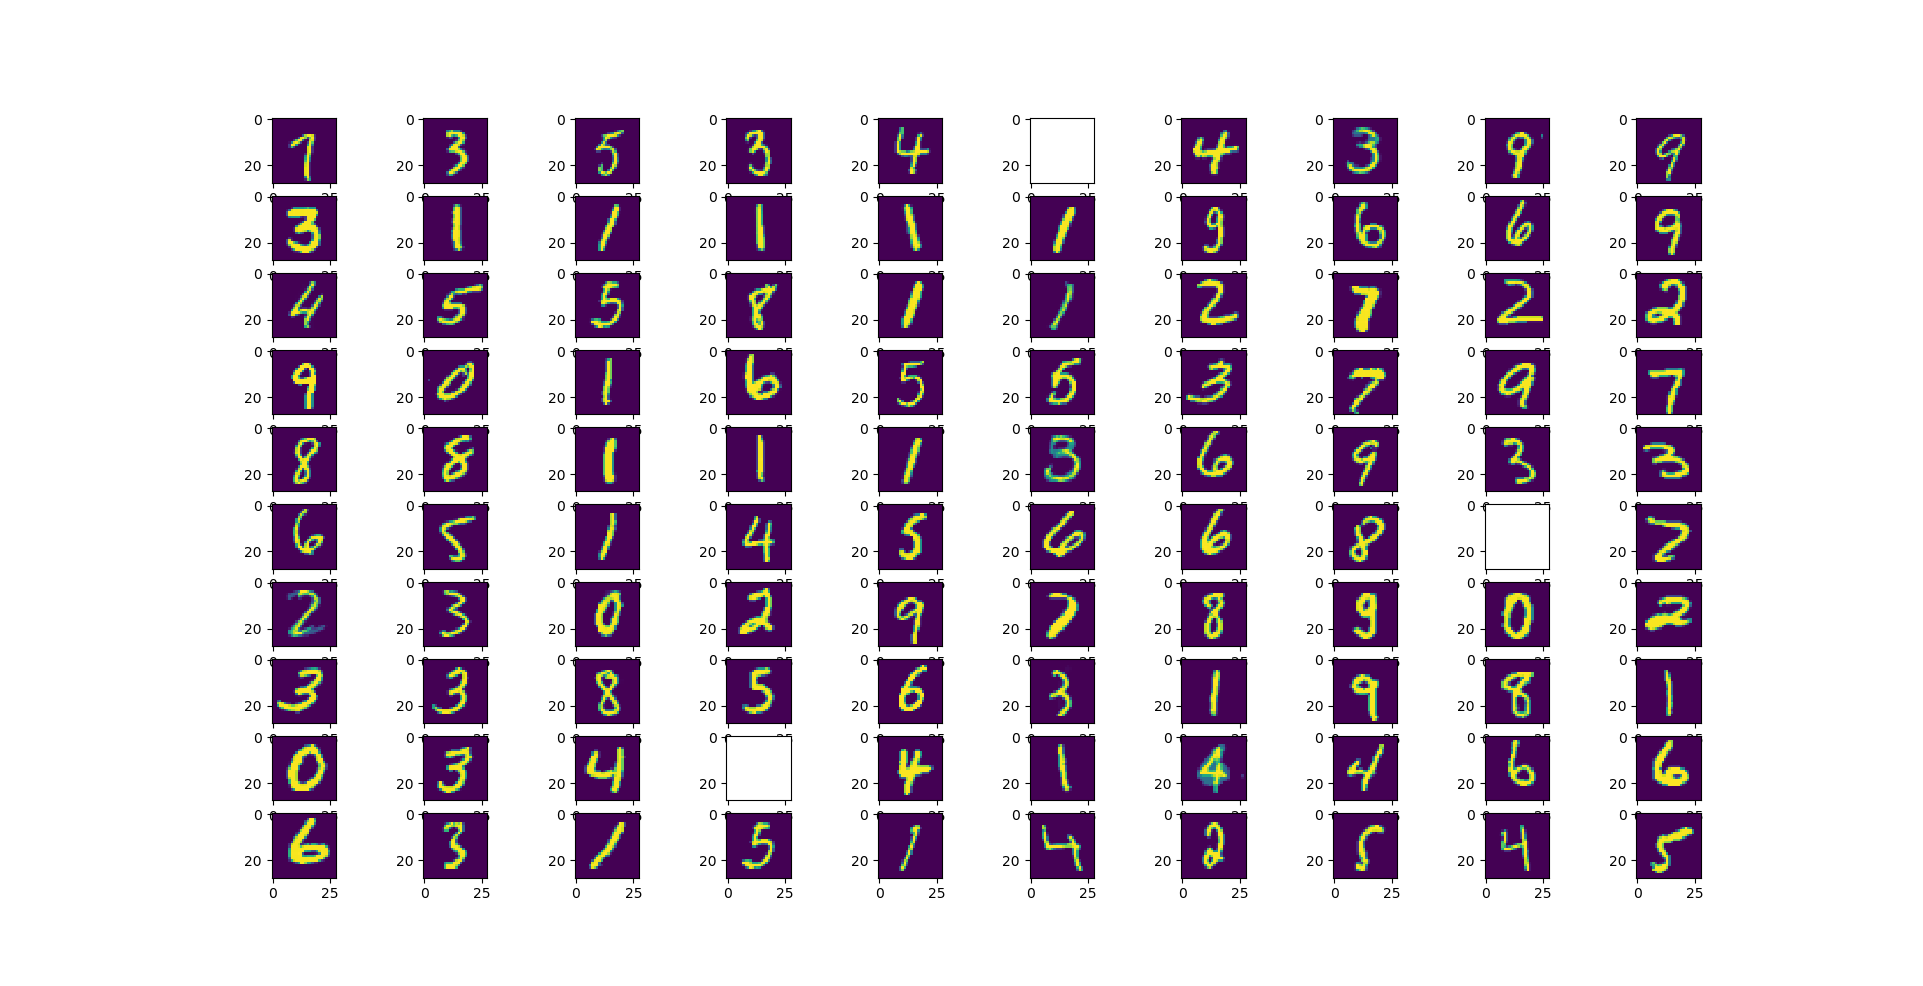
\includegraphics[width=\linewidth]{sigma_025_cm.png}
  \caption{Result of CM algo with sigma 0.25.}
  \label{fig:cm025}
\end{figure}

\begin{figure}[h]
  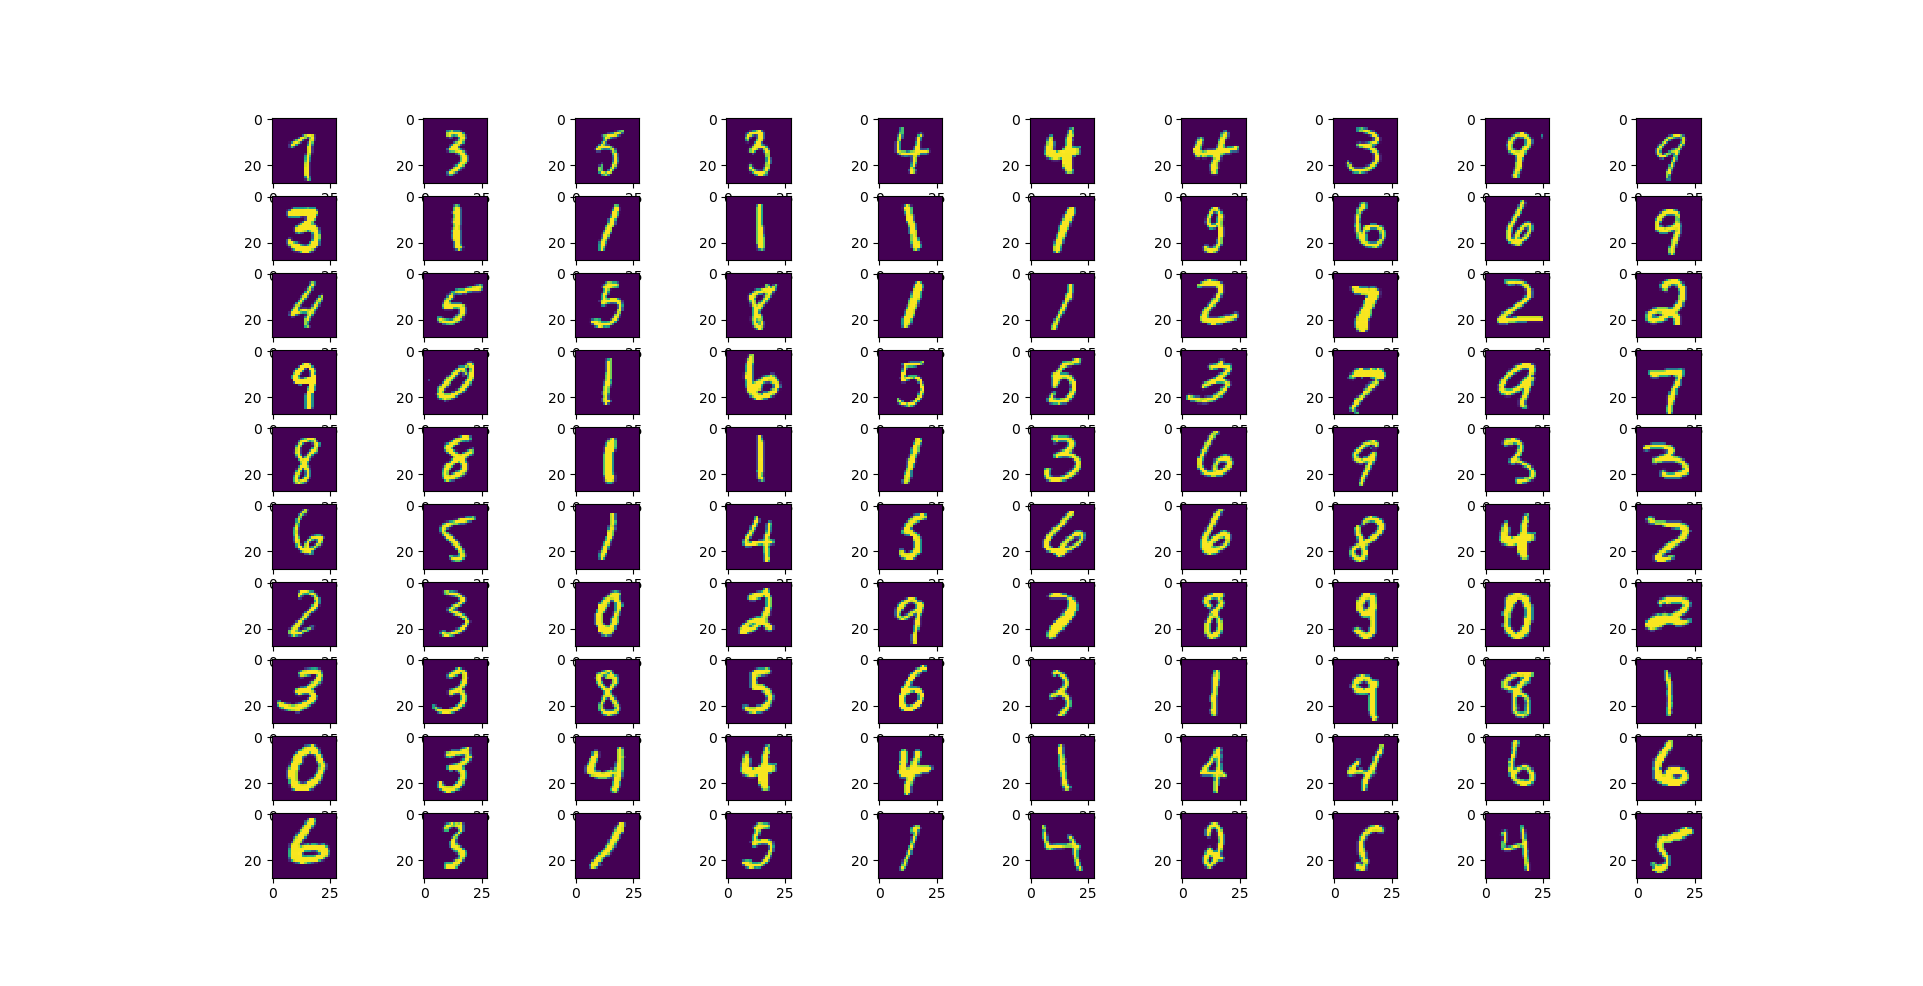
\includegraphics[width=\linewidth]{sigma_025_map.png}
  \caption{Result of MAP algo with sigma 0.25.}
  \label{fig:map025}
\end{figure}
As can be seen in figure \ref{fig:cm025} the CM algorithm did a pretty good job at removing the noise. There are only a few images, where the noise was not removed completely (e.g. the 3 at position x=6,y=5, where the algorithm almost made an 8 out of the 3) The MAP algorithm, however, did an excellent job, as can be seen in figure \ref{fig:map025}.
\pagebreak

\subsection{Sigma with 0.50}
\begin{figure}[!h]
  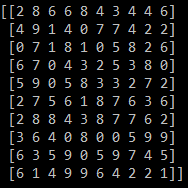
\includegraphics[width=\linewidth]{sigma_050_sol.png}
  \caption{Labels.}
  \label{fig:sol050}
\end{figure}

The labels for the choosen images can be seen in figure \ref{fig:sol050}.
\begin{figure}[h]
  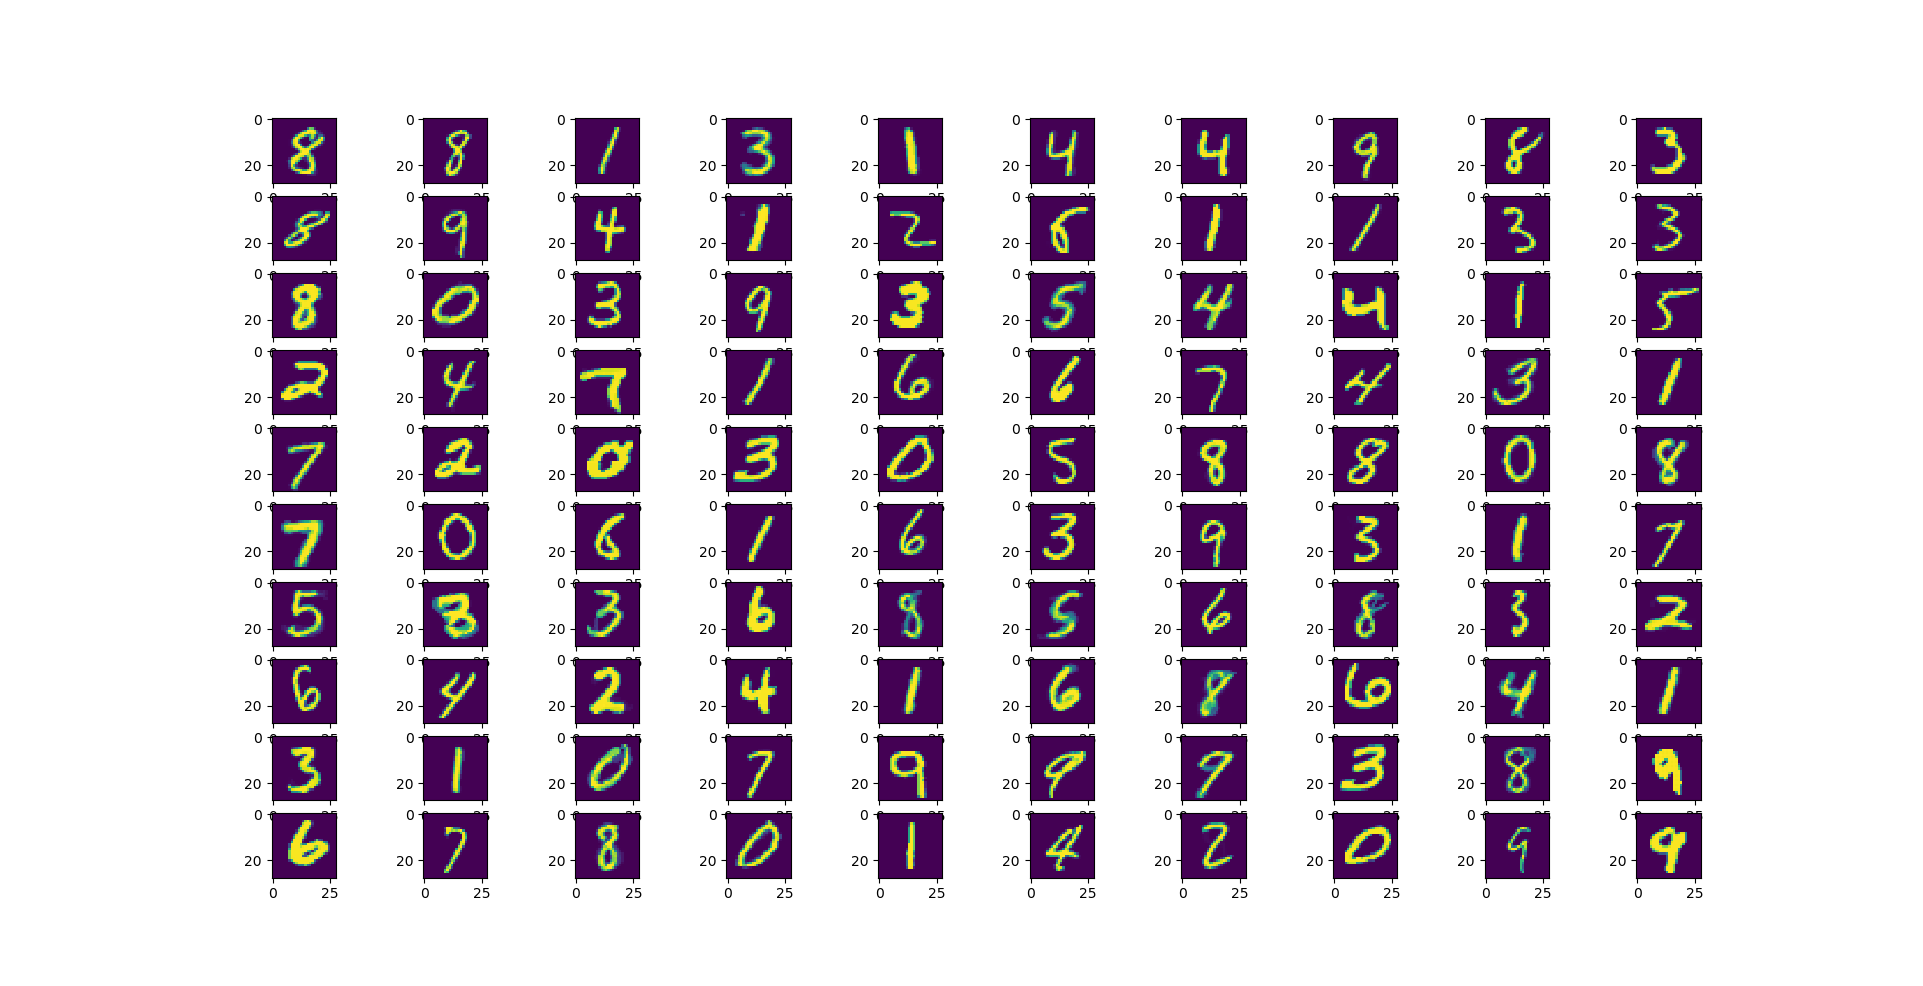
\includegraphics[width=\linewidth]{sigma_050_cm.png}
  \caption{Result of CM algo with sigma 0.50.}
  \label{fig:cm050}
\end{figure}

\begin{figure}[h]
  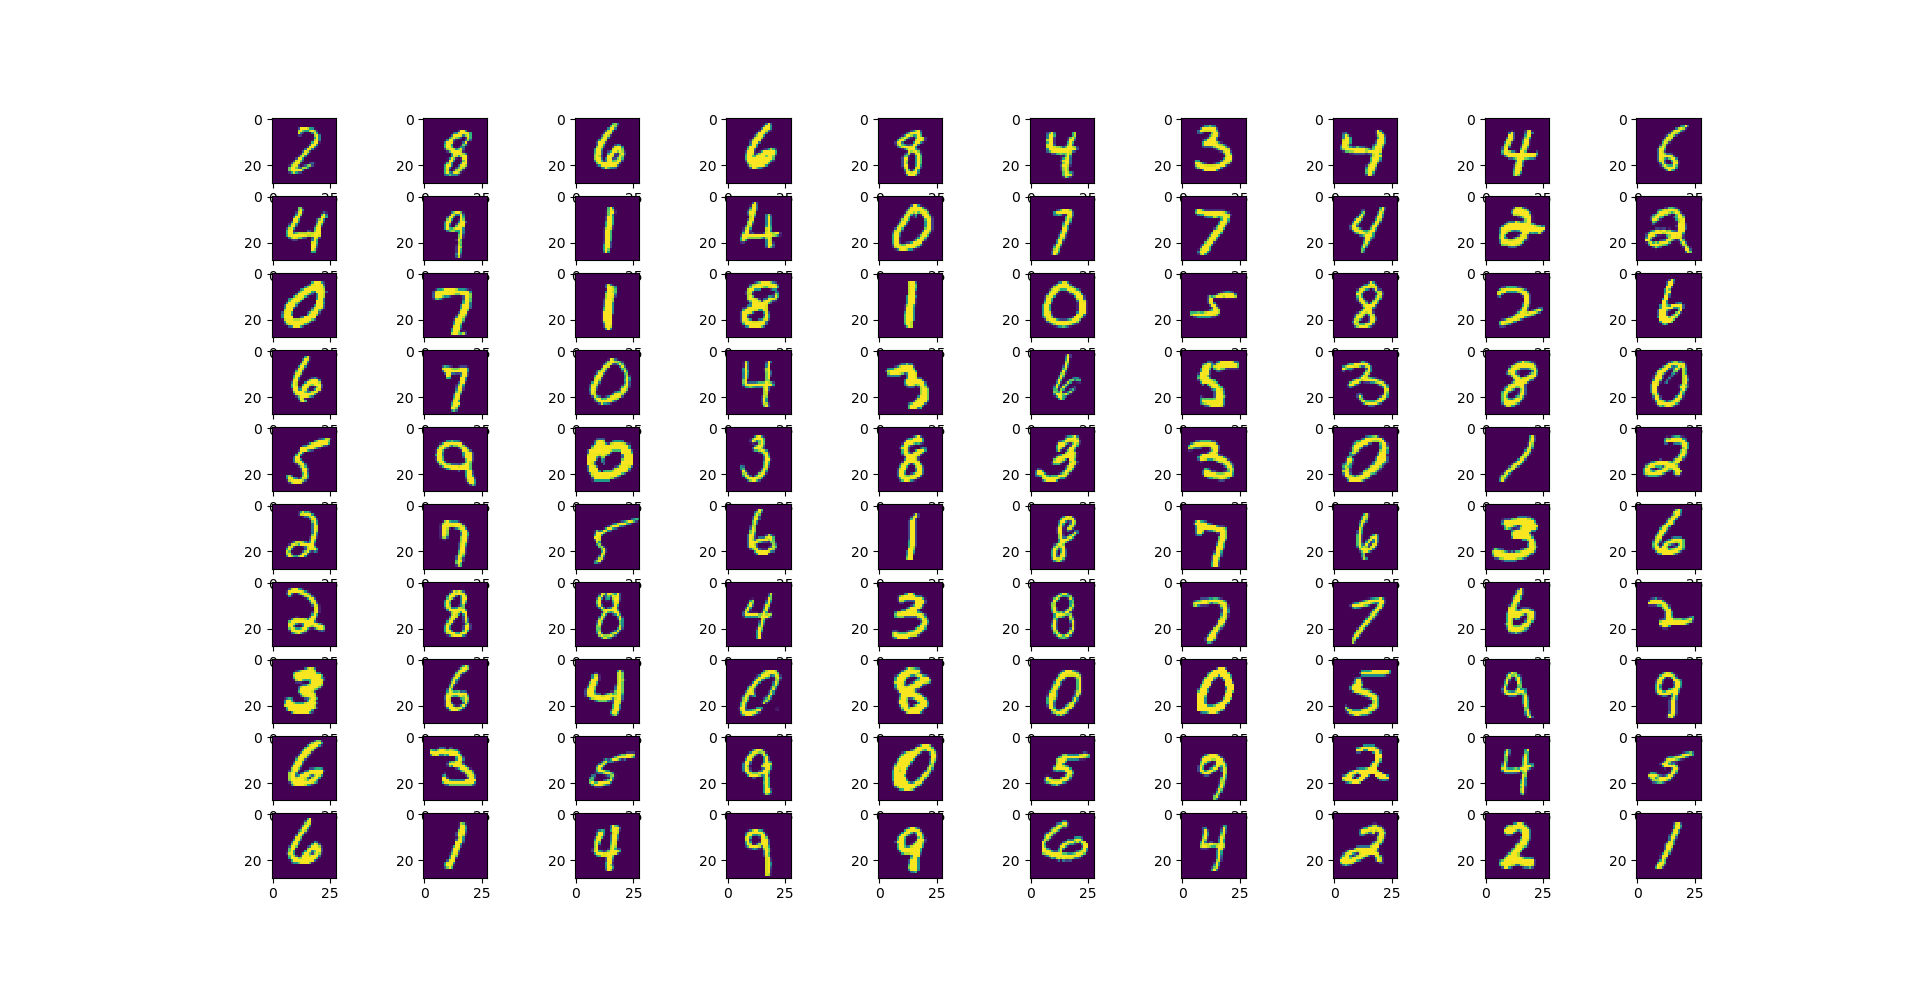
\includegraphics[width=\linewidth]{sigma_050_map.png}
  \caption{Result of MAP algo with sigma 0.50.}
  \label{fig:map050}
\end{figure}

As can be seen in figure \ref{fig:map050} for a sigma of 0.5 the MAP algo again did a very good job. All noisy images were correctly assigned. And while the mc algo performed good as well, the results are a bit different, as can be seen in figure \ref{fig:cm050}. The algorithm connected lines which were disconnected in the original image (e.g. the sloppy 8 at position x=6;y=6 or the sloppy 9 at position x=9;x=8) and thickened lines, which were thin (because of the pen pressure) in the origiinal image (e.g. the 5 at position x=3;y=9 or the 8 at position x=3;y=7)
\pagebreak
\subsection{Sigma with 1.00}
\begin{figure}[!h]
  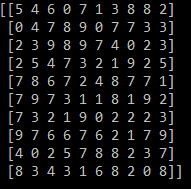
\includegraphics[width=\linewidth]{sigma_100_sol.png}
  \caption{Labels.}
  \label{fig:sol100}
\end{figure}
The labels for the choosen images can be seen in figure \ref{fig:sol050}.

\begin{figure}[h]
  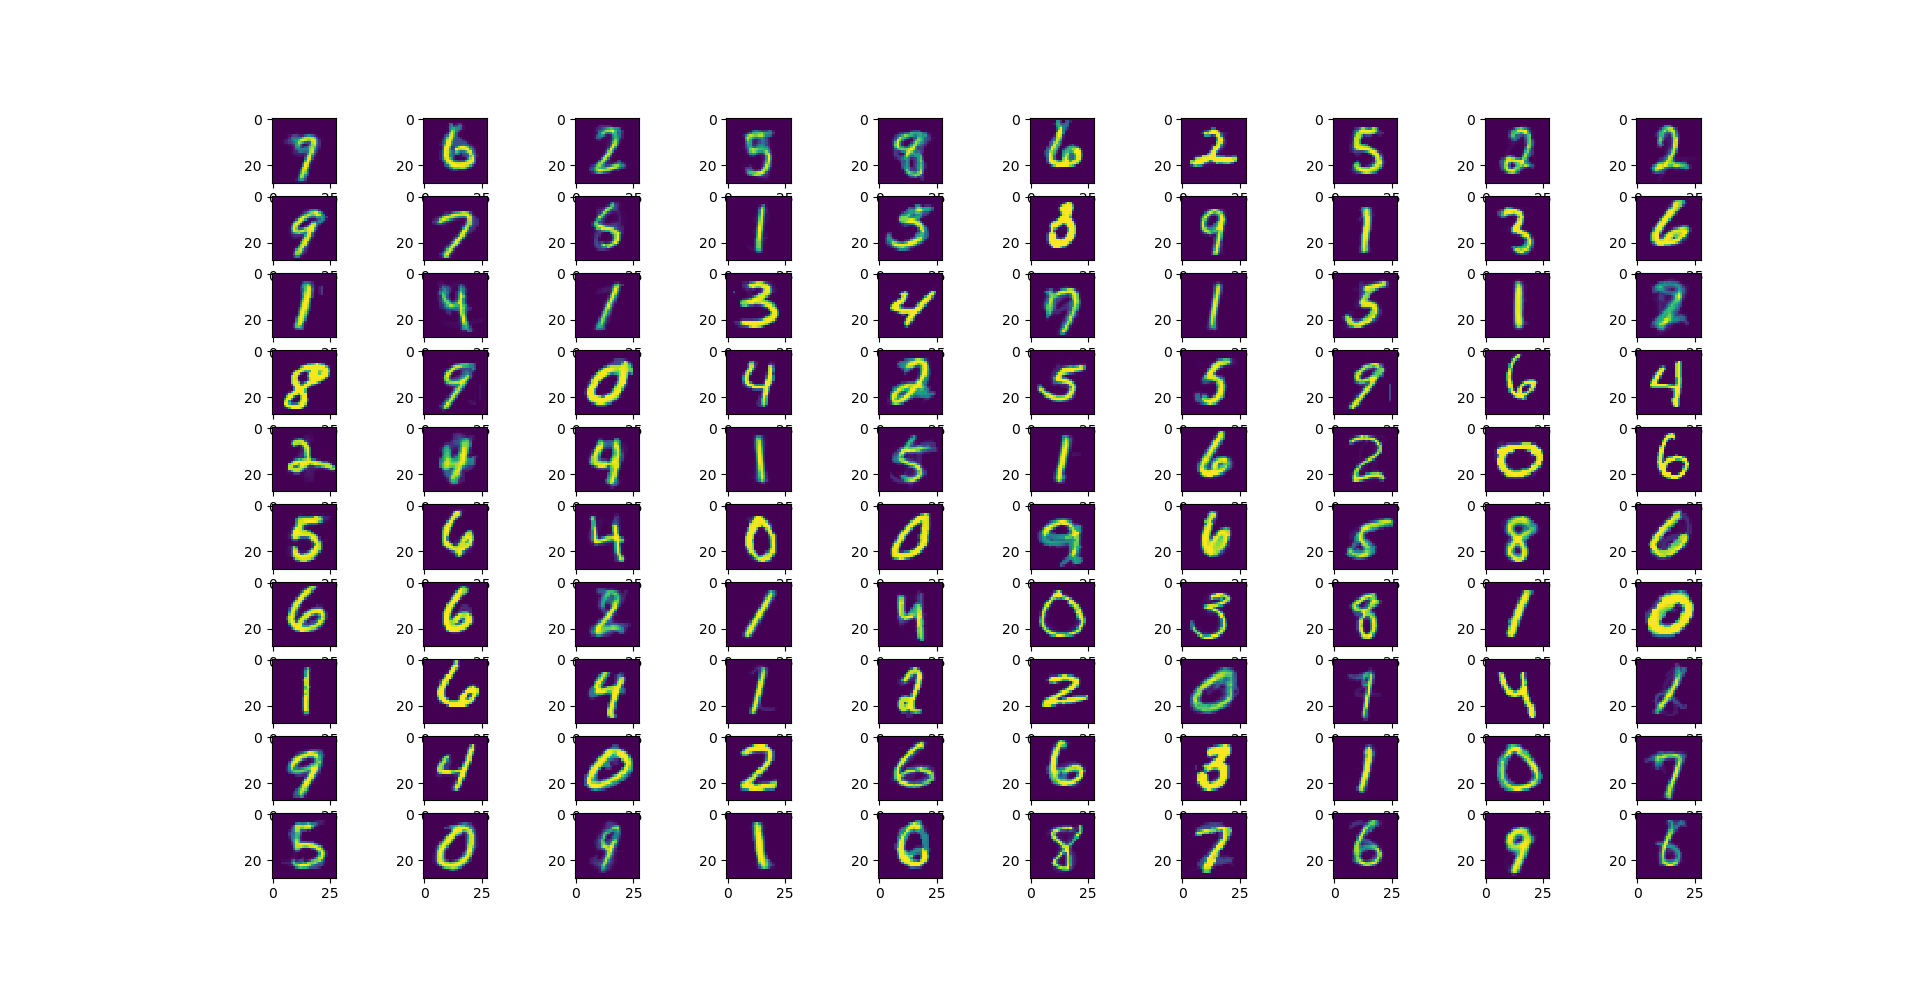
\includegraphics[width=\linewidth]{sigma_100_cm.png}
  \caption{Result of CM algo with sigma 1.}
  \label{fig:cm100}
\end{figure}

\begin{figure}[h]
  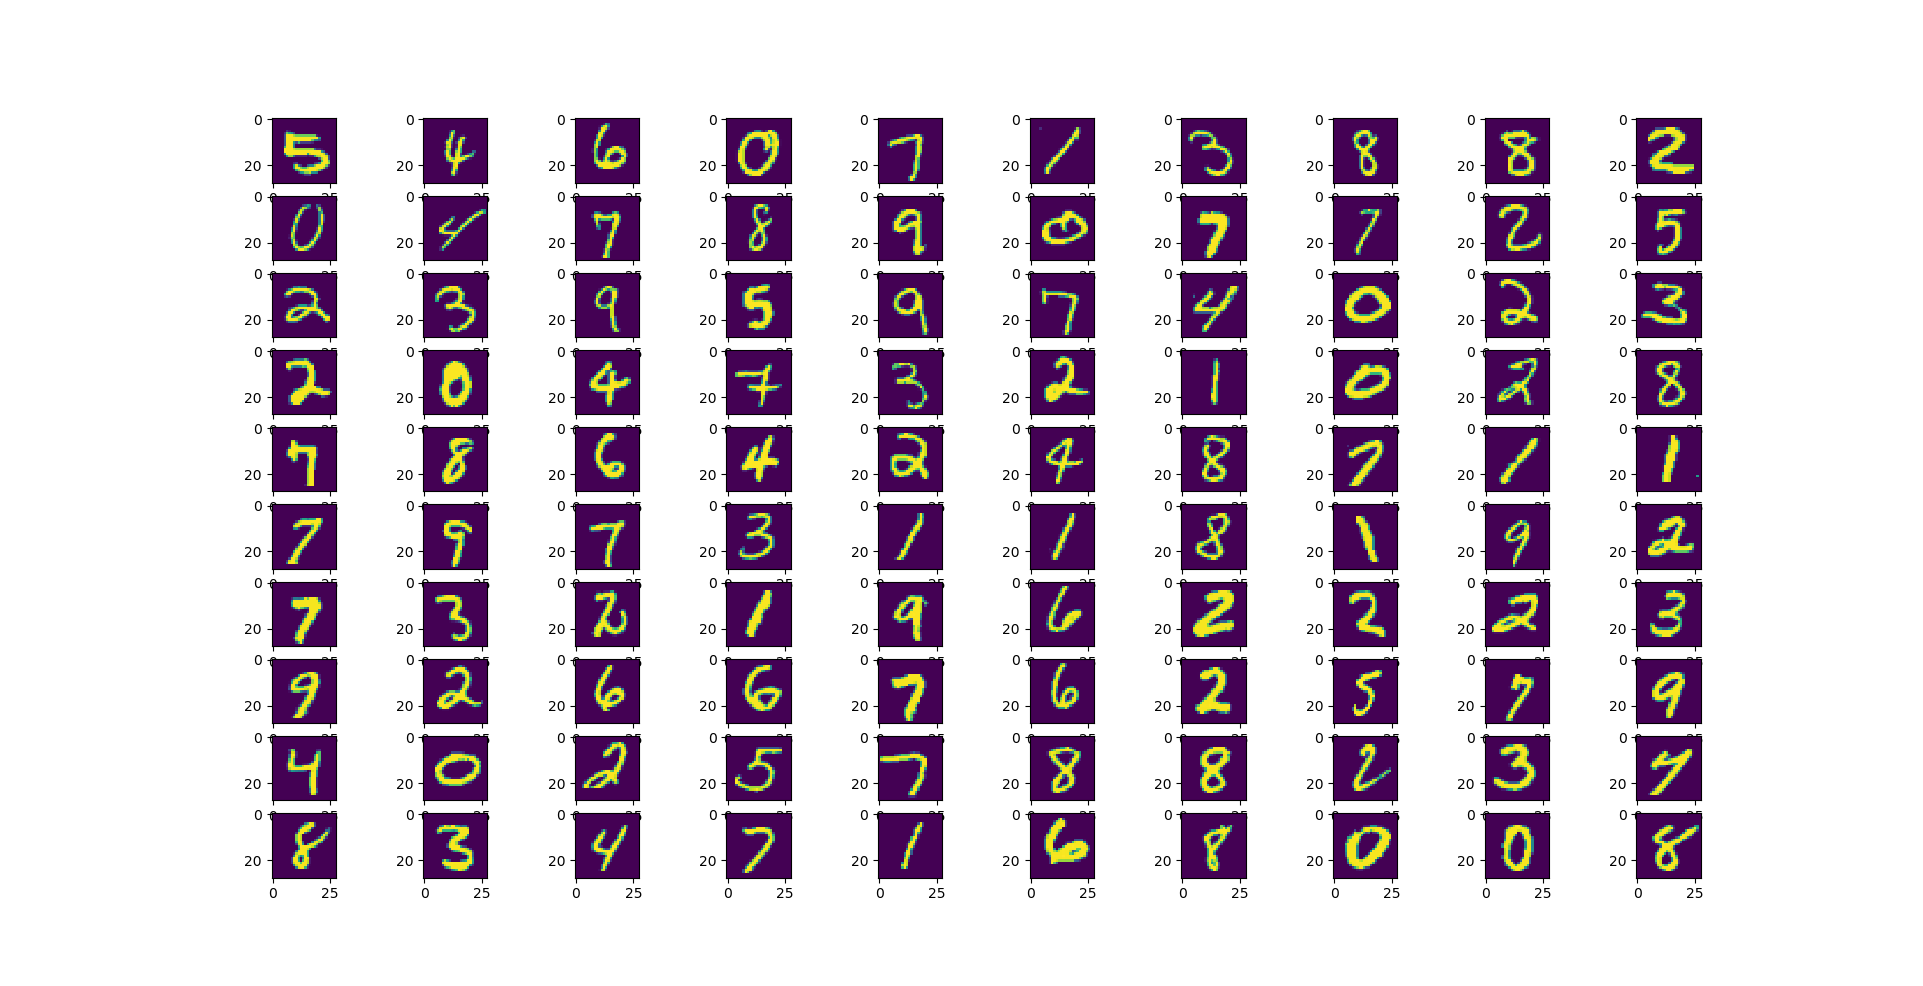
\includegraphics[width=\linewidth]{sigma_100_map.png}
  \caption{Result of MAP algo with sigma 1.0.}
  \label{fig:map100}
\end{figure}

With a larger sigma, the MAP algo did multiple misassignments, as can be seen in figure \ref{fig:map100}, if one compares the images to the ground truth labels. More than 15\% of the images are misassigned, in addition, none of the numbers which were misassigned resemble each other (e.g. 0 instead of 2 at position x=8;y=10)
The results for the CM algo, which can be seen in figure \ref{fig:cm100} are as worse as we expected for a sigma of 1.0. Most of the images have a lot of noise in it, some even have traces of other numbers mixed in. (e.g. the 3, where the noise resembles a 9 at position x=2;y=3)

Which brings following conclusion: Both algorithms don't work too well with a lot of noise, however, if the noise is small both work pretty well!
\pagebreak

\subsection{Differences between CM and MAP}
The MAP algorithm returns the image with the highest probability - the image the noisy image resembles the most. The CM algorithm however considers all the images which resemble the noisy image (= images with a high probability weight more than images with a low one) and reconstructs the image by taking the mean of all images.

\clearpage
\section{plots}
\label{plots}
\subsection{Task 2}
\subsubsection{Bivariate Gaussian}

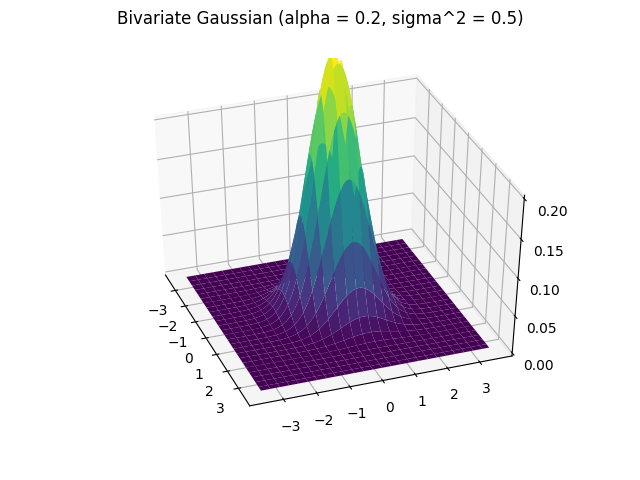
\includegraphics[width=\linewidth]{Bivariate Gaussian (alpha = 0.2, sigma^2 = 0.5).png}
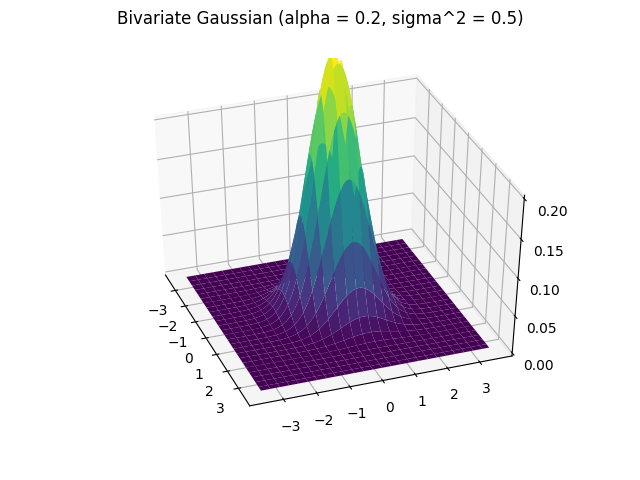
\includegraphics[width=\linewidth]{Bivariate Gaussian (alpha = 0.2, sigma^2 = 0.5).png}
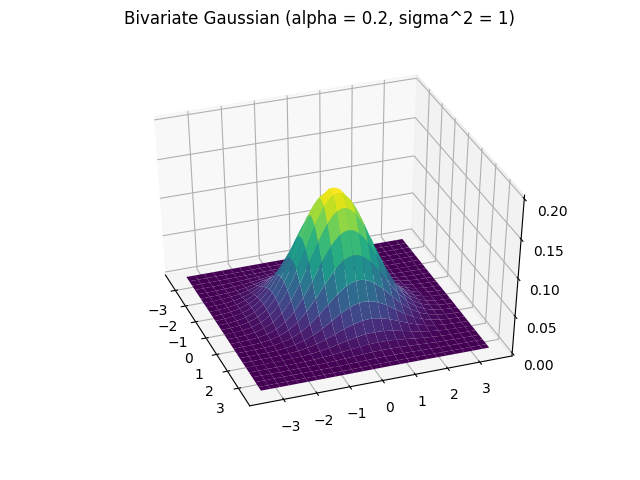
\includegraphics[width=\linewidth]{Bivariate Gaussian (alpha = 0.2, sigma^2 = 1).png}
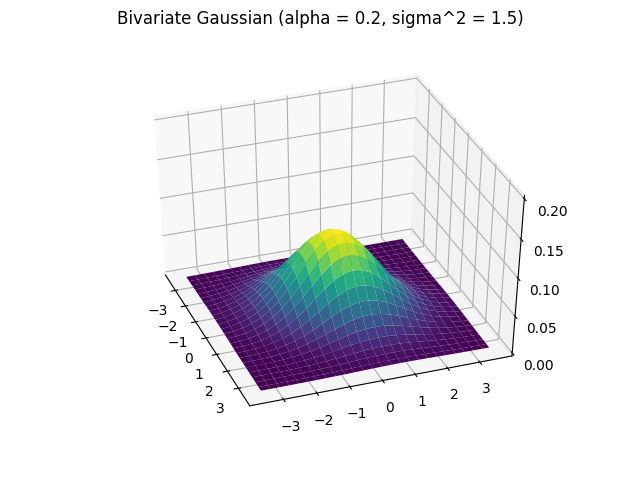
\includegraphics[width=\linewidth]{Bivariate Gaussian (alpha = 0.2, sigma^2 = 1.5).png}
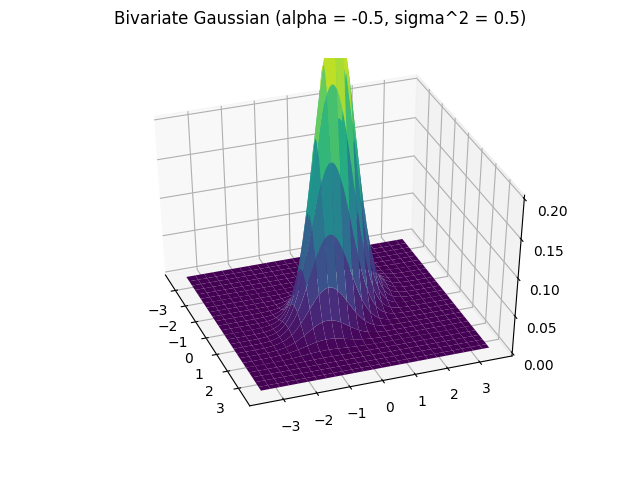
\includegraphics[width=\linewidth]{Bivariate Gaussian (alpha = -0.5, sigma^2 = 0.5).png}
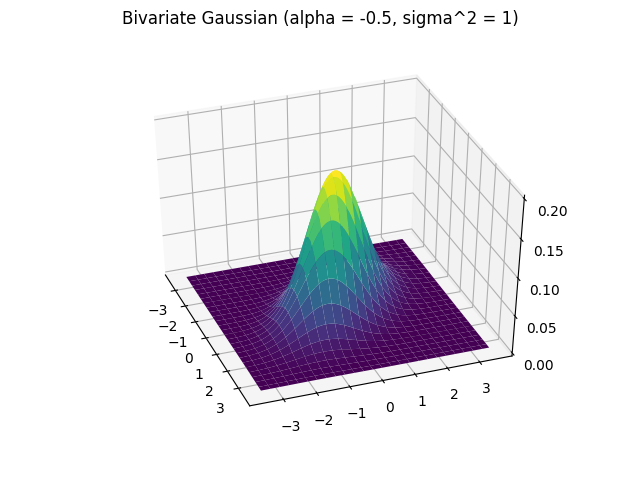
\includegraphics[width=\linewidth]{Bivariate Gaussian (alpha = -0.5, sigma^2 = 1).png}
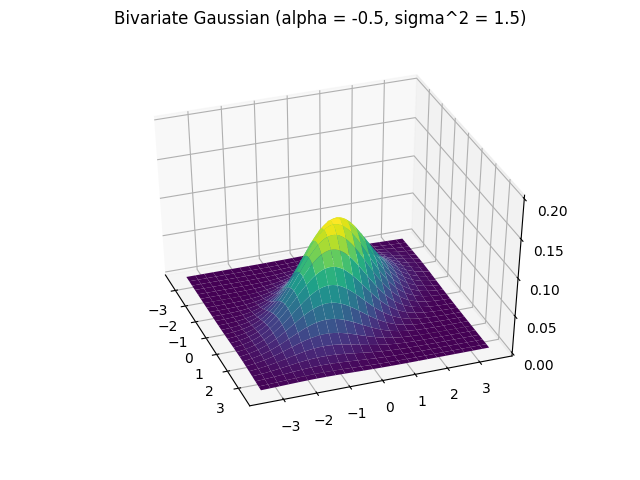
\includegraphics[width=\linewidth]{Bivariate Gaussian (alpha = -0.5, sigma^2 = 1.5).png}
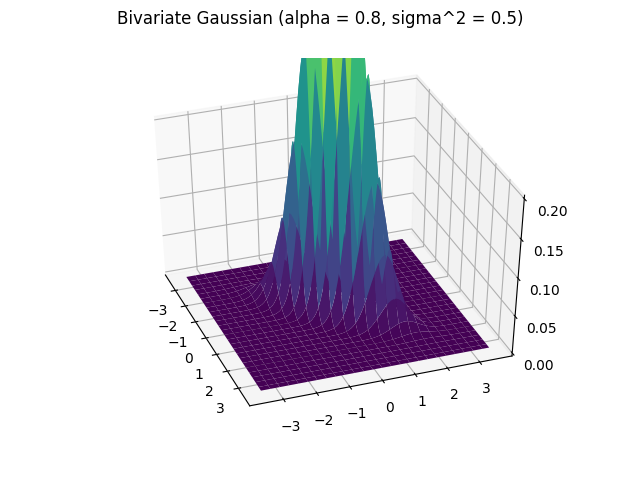
\includegraphics[width=\linewidth]{Bivariate Gaussian (alpha = 0.8, sigma^2 = 0.5).png}
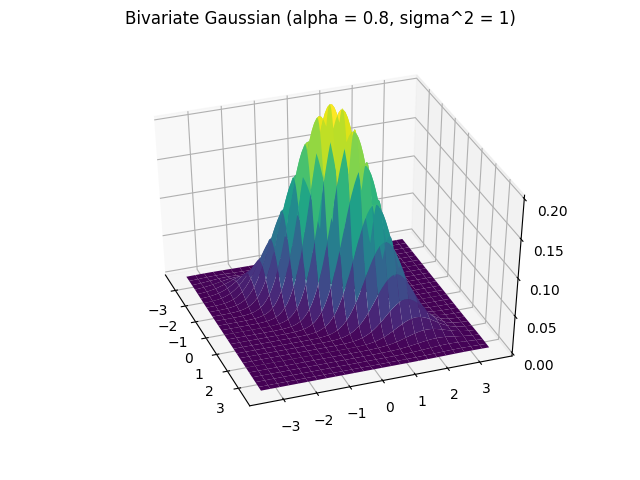
\includegraphics[width=\linewidth]{Bivariate Gaussian (alpha = 0.8, sigma^2 = 1).png}
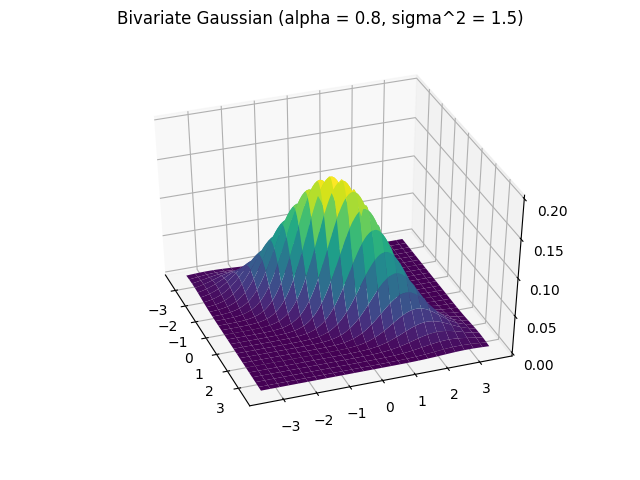
\includegraphics[width=\linewidth]{Bivariate Gaussian (alpha = 0.8, sigma^2 = 1.5).png}

\subsubsection{Bivariate Gaussian Marginals}
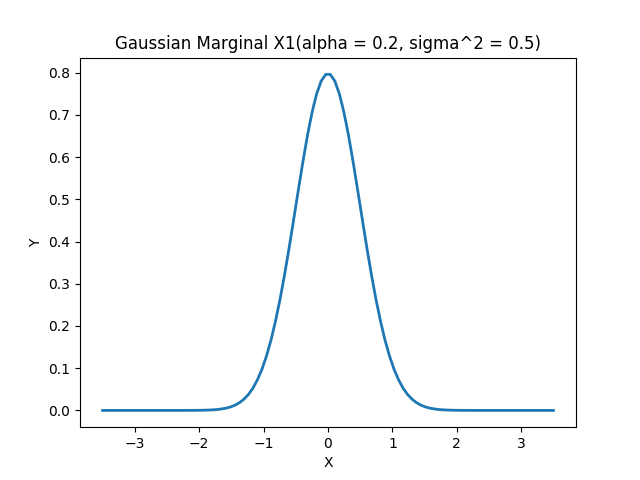
\includegraphics[width=\linewidth]{X1(alpha = 0.2, sigma^2 = 0.5).png}
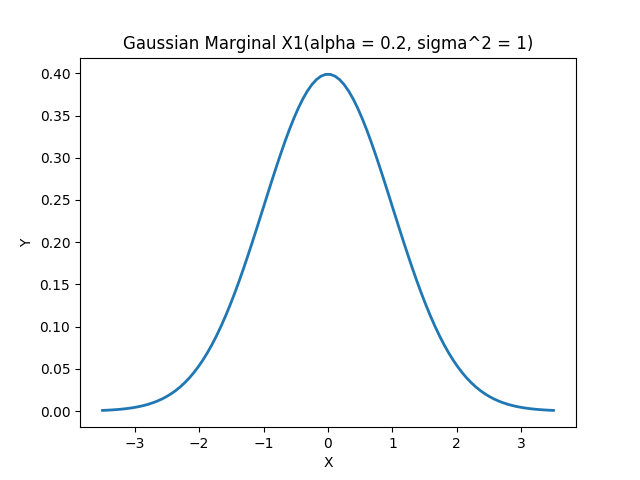
\includegraphics[width=\linewidth]{X1(alpha = 0.2, sigma^2 = 1).png}
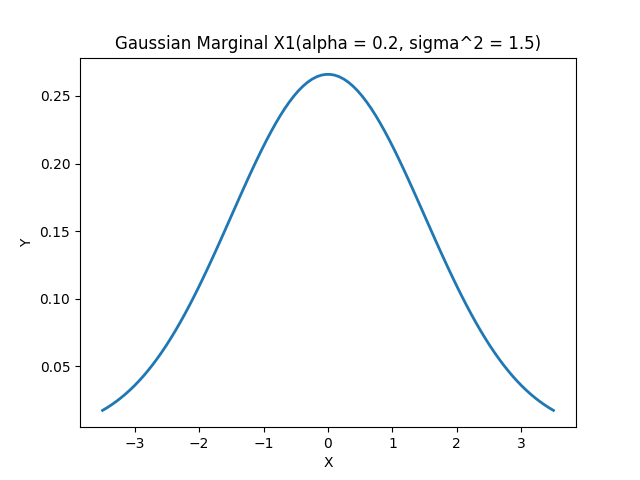
\includegraphics[width=\linewidth]{X1(alpha = 0.2, sigma^2 = 1.5).png}
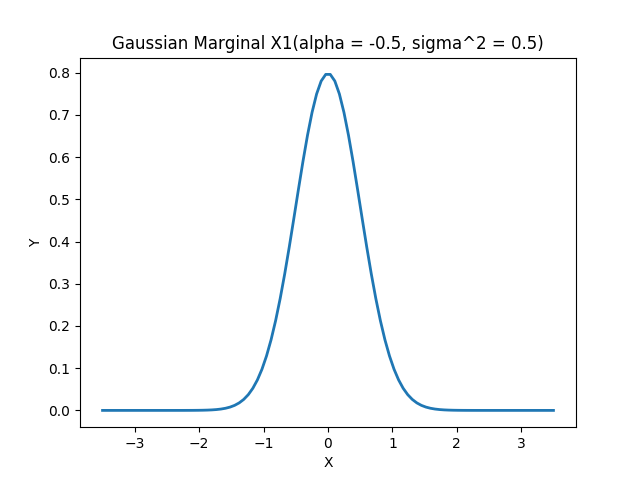
\includegraphics[width=\linewidth]{X1(alpha = -0.5, sigma^2 = 0.5).png}
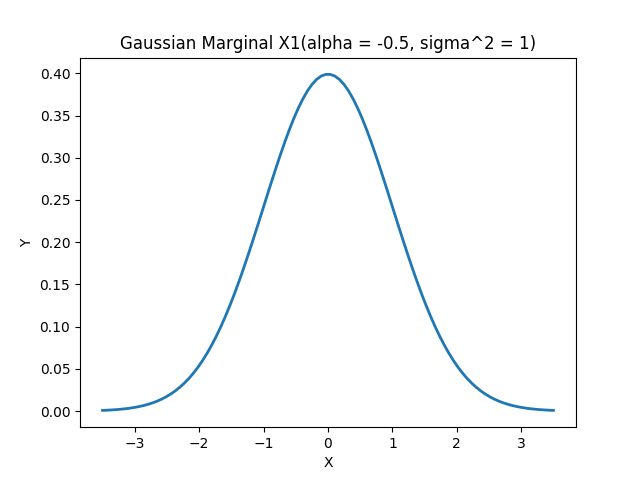
\includegraphics[width=\linewidth]{X1(alpha = -0.5, sigma^2 = 1).png}
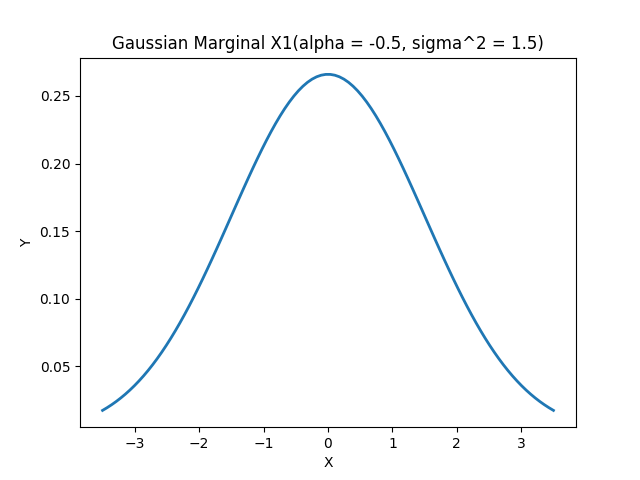
\includegraphics[width=\linewidth]{X1(alpha = -0.5, sigma^2 = 1.5).png}
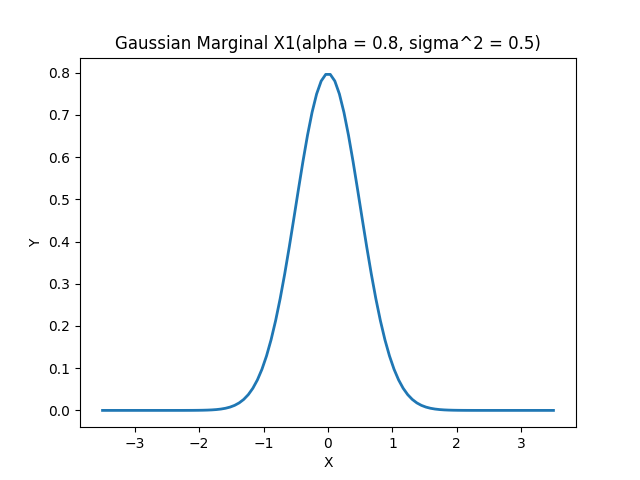
\includegraphics[width=\linewidth]{X1(alpha = 0.8, sigma^2 = 0.5).png}
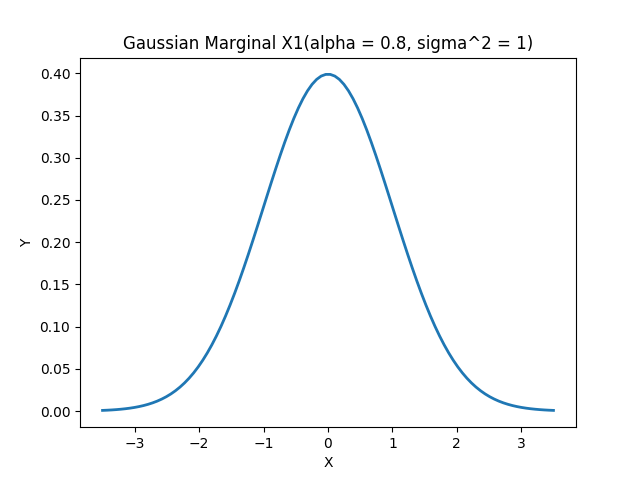
\includegraphics[width=\linewidth]{X1(alpha = 0.8, sigma^2 = 1).png}
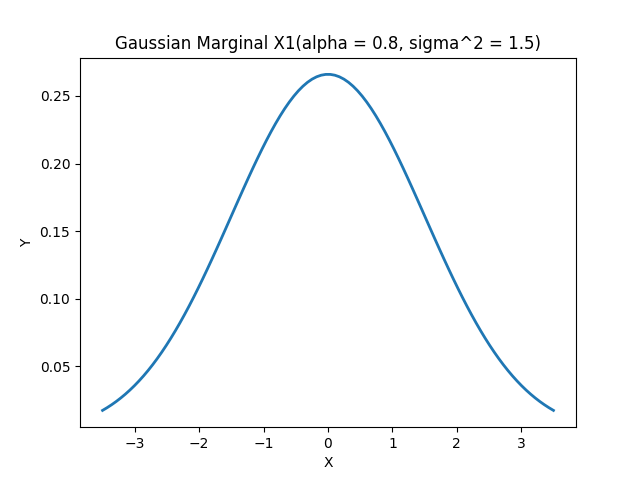
\includegraphics[width=\linewidth]{X1(alpha = 0.8, sigma^2 = 1.5).png}

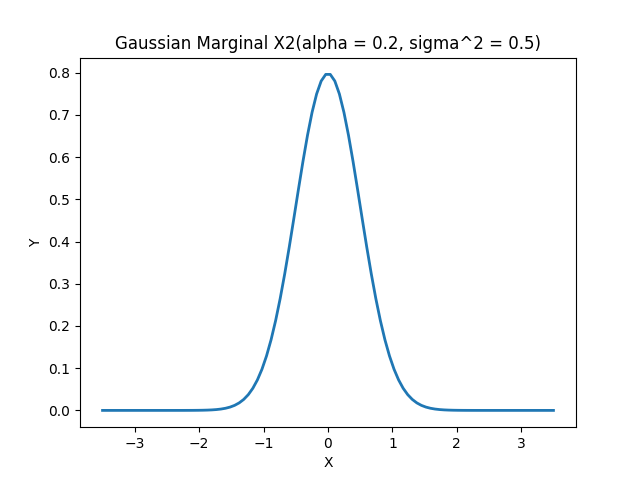
\includegraphics[width=\linewidth]{X2(alpha = 0.2, sigma^2 = 0.5).png}
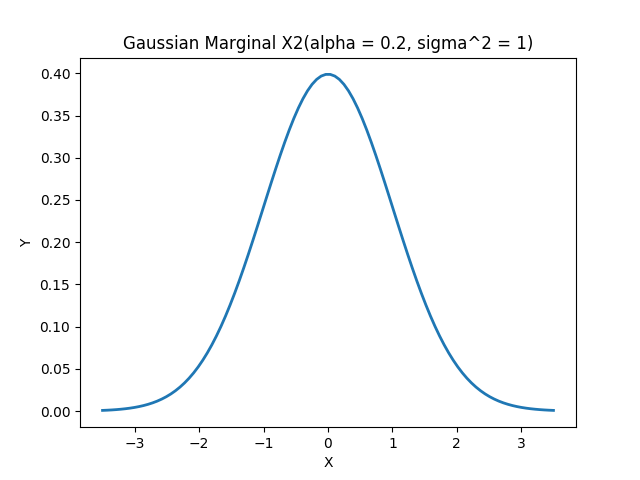
\includegraphics[width=\linewidth]{X2(alpha = 0.2, sigma^2 = 1).png}
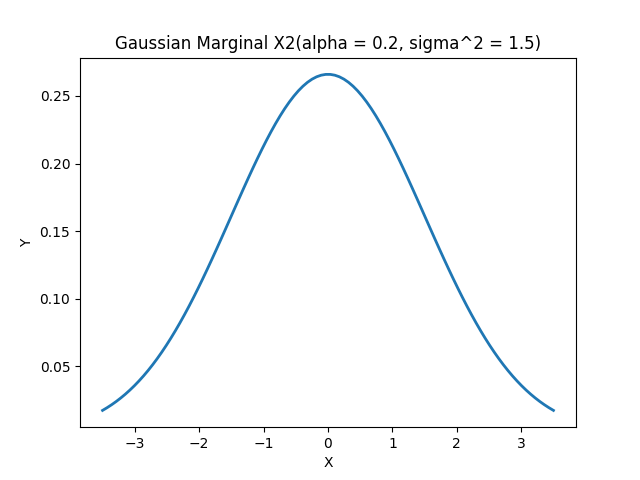
\includegraphics[width=\linewidth]{X2(alpha = 0.2, sigma^2 = 1.5).png}
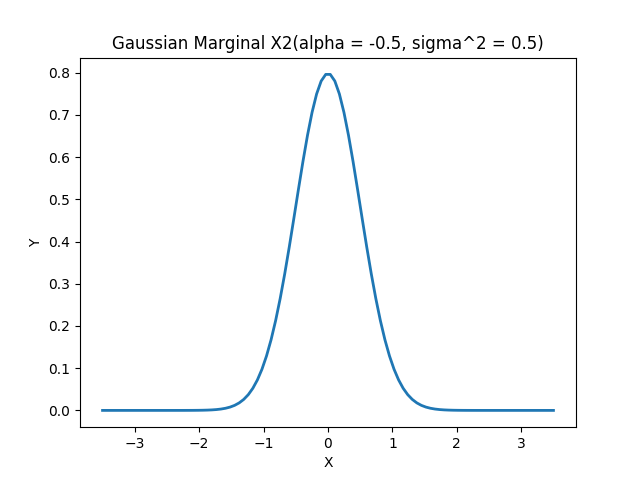
\includegraphics[width=\linewidth]{X2(alpha = -0.5, sigma^2 = 0.5).png}
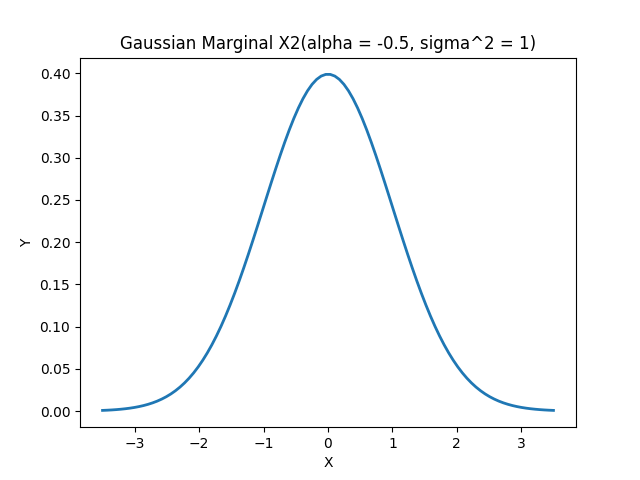
\includegraphics[width=\linewidth]{X2(alpha = -0.5, sigma^2 = 1).png}
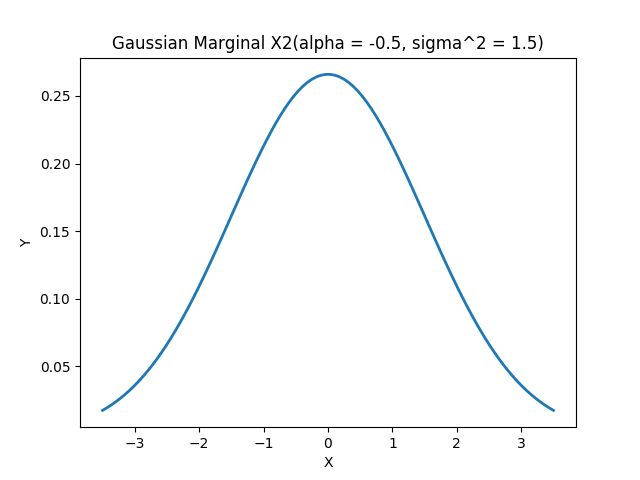
\includegraphics[width=\linewidth]{X2(alpha = -0.5, sigma^2 = 1.5).png}
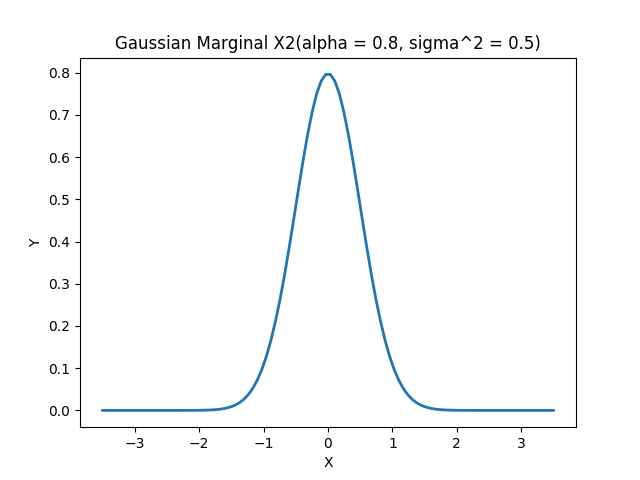
\includegraphics[width=\linewidth]{X2(alpha = 0.8, sigma^2 = 0.5).png}
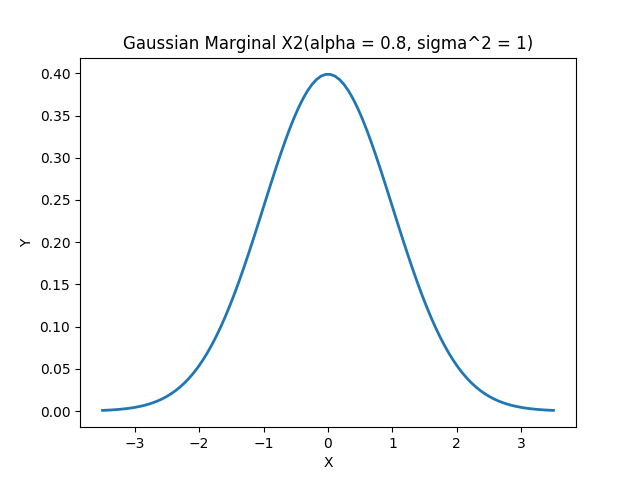
\includegraphics[width=\linewidth]{X2(alpha = 0.8, sigma^2 = 1).png}
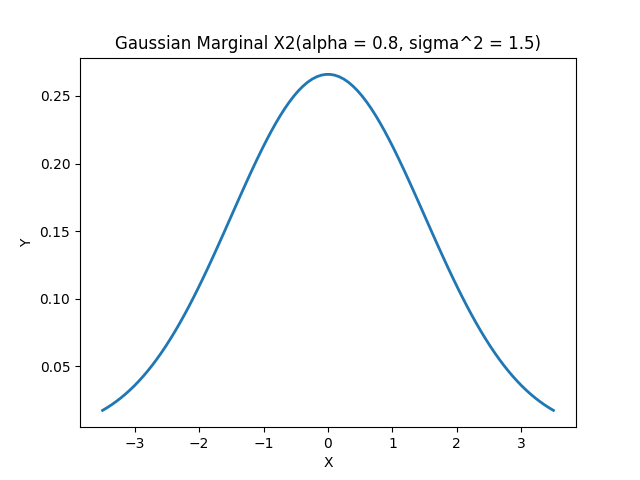
\includegraphics[width=\linewidth]{X2(alpha = 0.8, sigma^2 = 1.5).png}

\subsection{Task 3}
\subsubsection{Model Predictions}
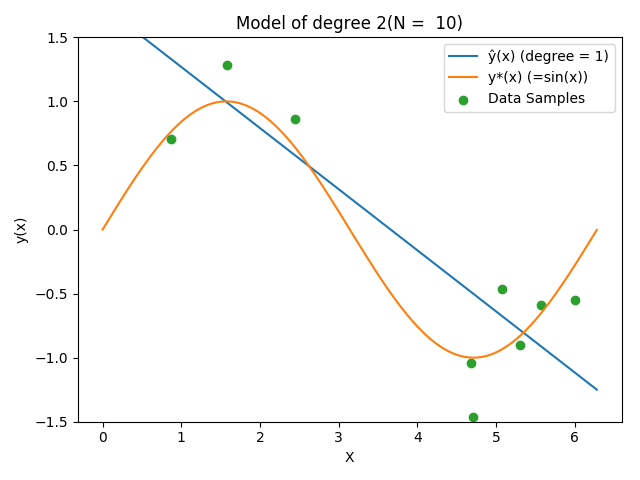
\includegraphics[width=\linewidth]{2.png}
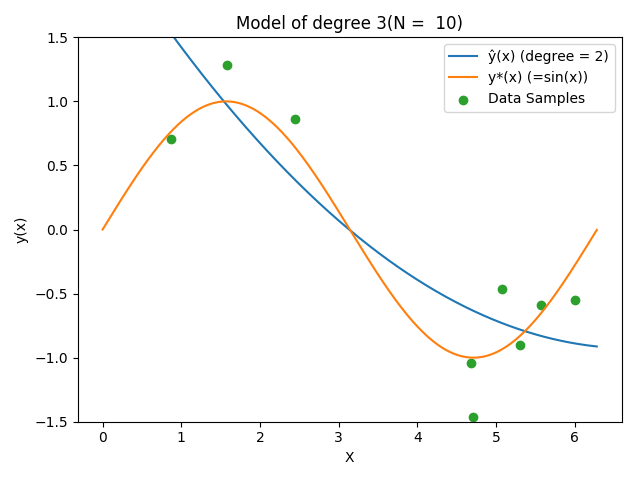
\includegraphics[width=\linewidth]{3.png}
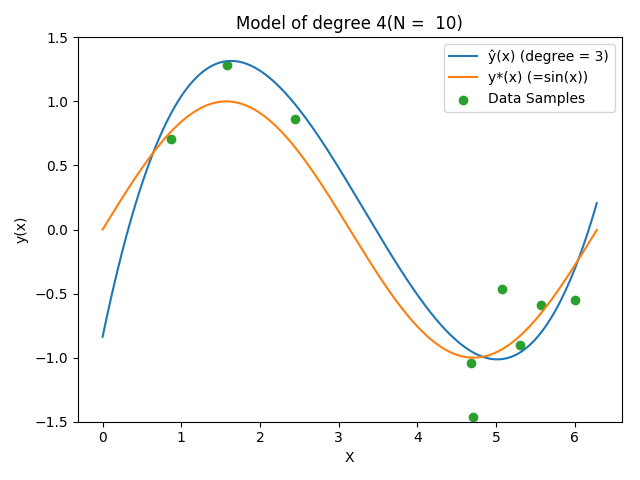
\includegraphics[width=\linewidth]{4.png}
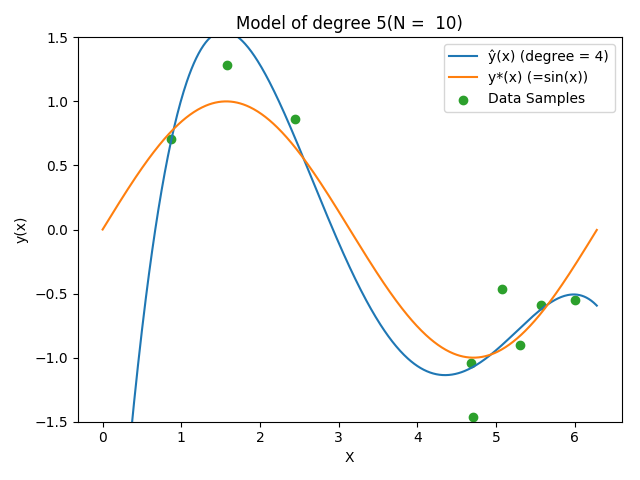
\includegraphics[width=\linewidth]{5.png}
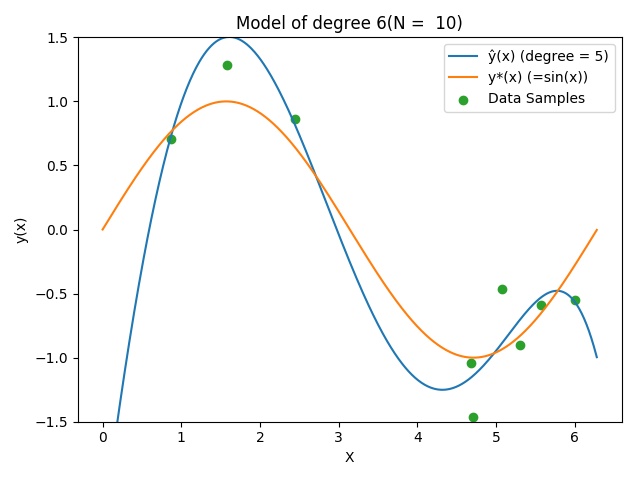
\includegraphics[width=\linewidth]{6.png}
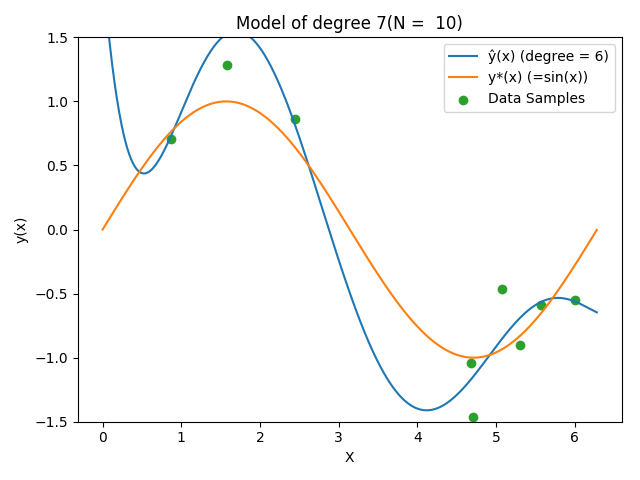
\includegraphics[width=\linewidth]{7.png}
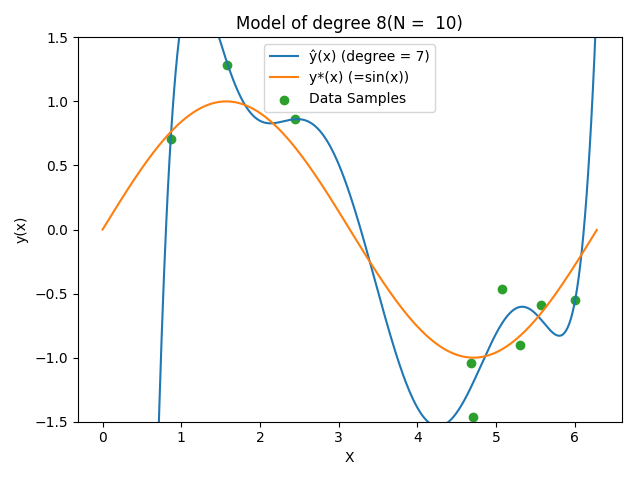
\includegraphics[width=\linewidth]{8.png}
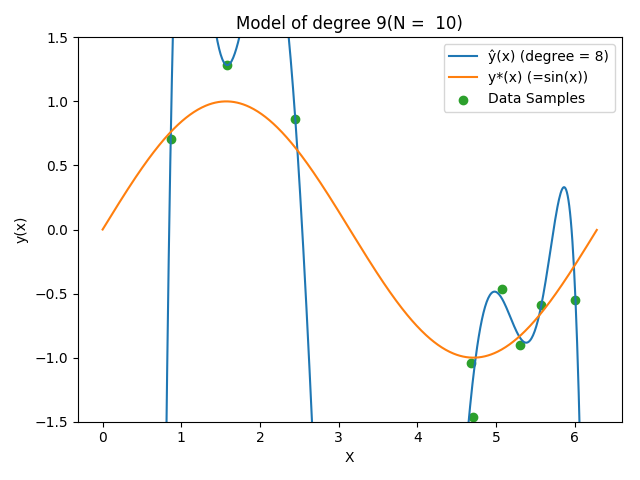
\includegraphics[width=\linewidth]{9.png}

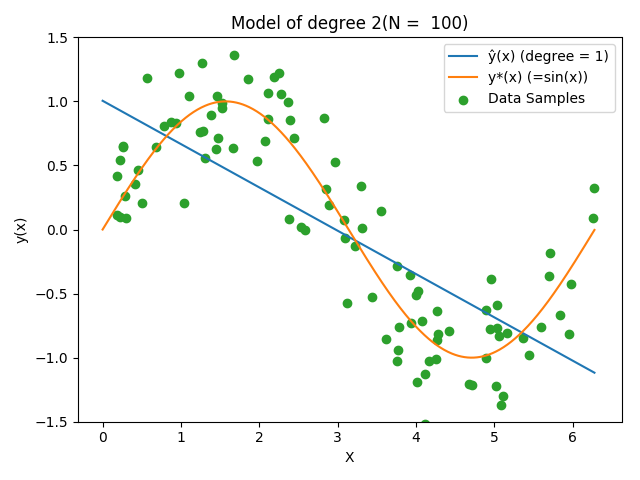
\includegraphics[width=\linewidth]{2_100.png}
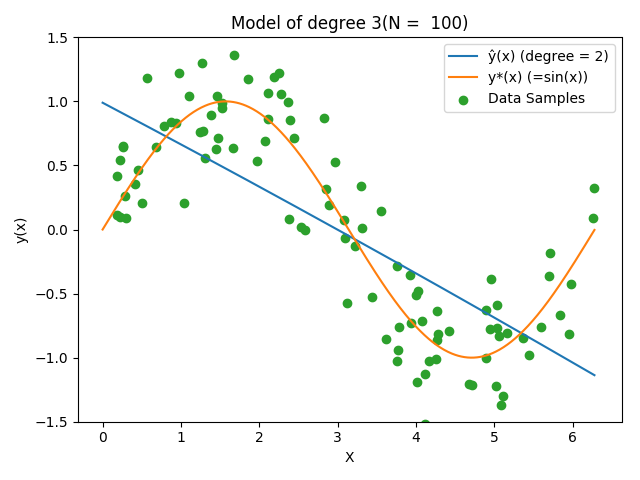
\includegraphics[width=\linewidth]{3_100.png}
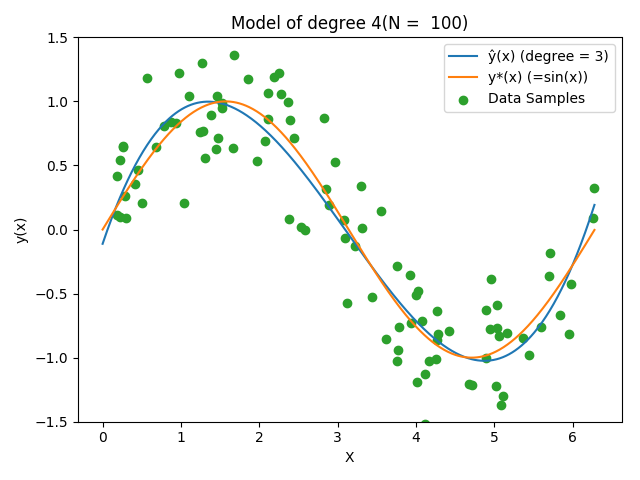
\includegraphics[width=\linewidth]{4_100.png}
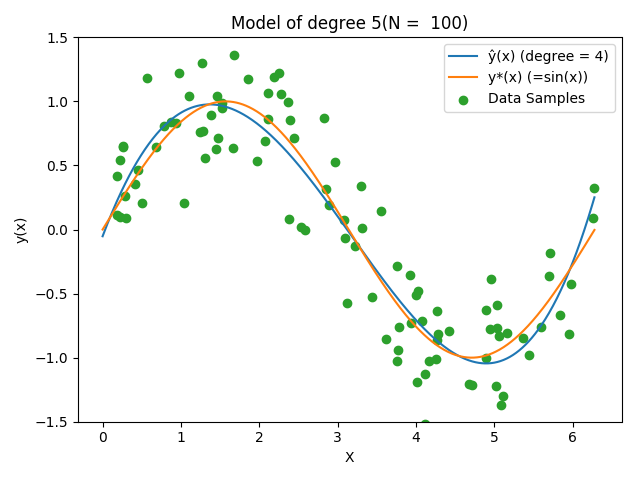
\includegraphics[width=\linewidth]{5_100.png}
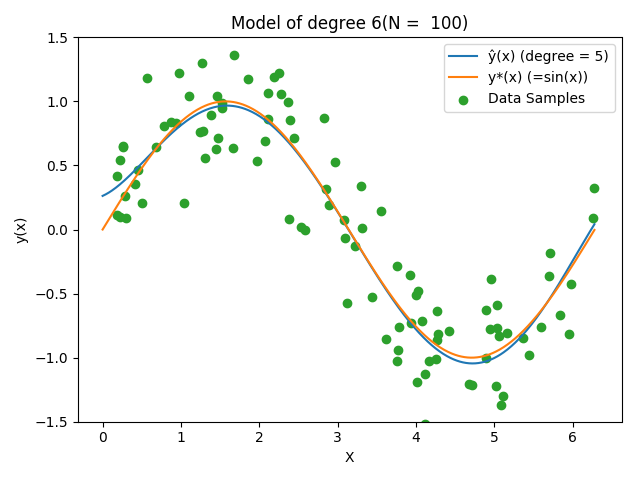
\includegraphics[width=\linewidth]{6_100.png}
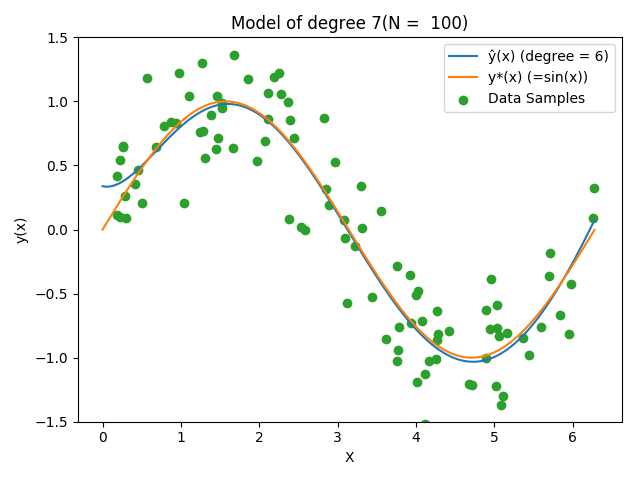
\includegraphics[width=\linewidth]{7_100.png}
\includegraphics[width=\linewidth]{8_100.png}
\includegraphics[width=\linewidth]{9_100.png}


\subsubsection{Risk}
\includegraphics[width=\linewidth]{empirical.png}
\includegraphics[width=\linewidth]{empirical_100.png}
\includegraphics[width=\linewidth]{true.png}
\includegraphics[width=\linewidth]{true_100.png}


\end{document}
